\documentclass[article,a4paper,12pt,brazil,sumario=tradicional]{abntex2}
\usepackage{titlesec}

\setcounter{secnumdepth}{4}

\titleformat{\paragraph}
{\normalfont\normalsize}{\theparagraph}{1em}{}

\usepackage{array}
\usepackage{subfig}
\usepackage[utf8]{inputenc}
\usepackage{indentfirst}
\usepackage{hyperref}
\usepackage[hyphenbreaks]{breakurl}
\usepackage[alf,abnt-etal-text=it]{abntex2cite}
\usepackage[brazil]{babel}
\usepackage[space]{grffile}
\graphicspath{ {./images/} }
\setlength{\parindent}{3em}

\newcolumntype{C}[1]{>{\centering\arraybackslash\hspace{0pt}}p{#1}}

\setlrmarginsandblock{3cm}{3cm}{*}
\setulmarginsandblock{3cm}{2cm}{*}
\checkandfixthelayout

\titleformat{\section}{\normalfont\normalsize\bfseries}{\thesection.}{1em}{\MakeUppercase}
\titleformat{\subsection}{\normalfont\normalsize}{\thesubsection.}{1em}{\MakeUppercase}
\titleformat{\subsubsection}{\normalfont\normalsize\bfseries}{\thesubsubsection.}{1em}{}

\renewenvironment{quotation}
  {\small\list{}{\rightmargin=0cm \leftmargin=2cm}%
   \item\relax}
  {\endlist}
  
\hypersetup{%
    pdfborder = {0 0 0}
}

\title{ {\Large Título\footnote{Trabalho de conclusão de curso apresentado ao curso de Bacharelado em Sistemas de Informação da Universidade Federal Fluminense como requisito parcial para conclusão do curso.}\\\\
\vspace{.2} 
\textit{Titulo}\\}}

\date{ }

\begin{document}

\textual

\begin{center}
{\Large Impacto orçamentário da inserção de canabidiol no tratamento para epilepsia no estado do Rio de Janeiro\footnote{Trabalho de conclusão de curso apresentado ao curso de Bacharelado em Sistemas de Informação da Universidade Federal Fluminense como requisito parcial para conclusão do curso.}

\textit{Budgetary impact of the insertion of cannabidiol in the treatment of epilepsy in the state of Rio de Janeiro}\\}
\end{center}
\vspace{.2cm} 

\begin{flushright}
Bruno Moraes Cotelo\footnote{Graduando do Curso de Sistemas de Informação - UFF, bruno\_cotelo@id.uff.br}

Tiago Rodrigues de Matos\footnote{Graduando do Curso de Sistemas de Informação - UFF, ti\_matos@id.uff.br}

Daniel Cardoso Moraes de Oliveira\footnote{Orientador - Instituto de Computação - UFF, danielcmo@ic.uff.br.} 

\end{flushright}

\vspace{\onelineskip}

\begin{center}
    \textbf{Resumo}
\end{center}

\vspace{-.3cm}

\noindent Este estudo investiga a maneira com que pacientes que sofrem de epilepsia transitaram de estado e tratamento no Rio de Janeiro entre 2014 e 2023, focando no Sistema Público de Saúde (SIASUS). O Objetivo principal é realizar uma projeção de custo de inserção do canabidiol (CBD) no tratamento público para um período de 5 anos.

\vspace{.4cm}
 
\noindent
\textbf{Palavras-chaves}: Epilepsia, Transição de estado, Rio de Janeiro, Sistema Público de Saúde (SIASUS), Custo de inserção, Canabidiol (CBD), Tratamento público, Projeção de custo.
 
\vspace{\onelineskip}

\begin{center}
    \textbf{Abstract}
\end{center}

\vspace{-.3cm}
\begin{hyphenrules}{english}
\noindent This study investigates how patients suffering from epilepsy transitioned through state and treatment in Rio de Janeiro between 2014 and 2023, focusing on the Public Health System (SIASUS). The main objective is to project the cost of integrating cannabidiol (CBD) into public treatment for a period of 5 years.
\end{hyphenrules}
\vspace{.4cm}
 
\noindent \textbf{Keywords}: Epilepsy, State transition, Rio de Janeiro, Public Health System (SIASUS), Cost of integration, Cannabidiol (CBD), Public treatment, Cost projection.

\vspace{.4cm}

\noindent \textbf{Aprovado em:} dd/mm/aaaa.~~~\textbf{Versão Final em:} dd/mm/aaaa

\section{Introdução}

O uso medicinal de substâncias derivadas da \textit{Cannabis sp.} tem ganhado destaque na última década. Enquanto o tetrahidrocanabinol (THC) é conhecido por provocar a maioria dos efeitos psicoativos, o canabidiol (CBD) tem sido amplamente estudado por seus benefícios terapêuticos. O CBD é reconhecido por suas propriedades anti-inflamatórias, analgésicas, ansiolíticas e anticonvulsivantes, sendo responsável por grande parte dos efeitos medicinais da planta.
https://www.ncbi.nlm.nih.gov/pmc/articles/PMC4604171/
https://www.ncbi.nlm.nih.gov/books/NBK425767/

No presente trabalho, um dos aspectos importantes a serem abordados é o uso do canabidiol (CBD) no tratamento de convulsões, especialmente aquelas crônicas causadas pelos diversos tipos de epilepsia. A epilepsia é um distúrbio neurológico caracterizado por crises espontâneas resultantes de atividade elétrica anormal no cérebro. Este grupo de distúrbios pode ser desencadeado por vários fatores. Atualmente, no Brasil, cerca de 3 milhões de pessoas sofrem de crises epilépticas, de acordo com a Secretaria de Saúde do Distrito Federal (Referenciar).

O uso e comercialização do produto no brasil era proscrito até o ano de xxxx, sendo liberado primeiramente pela anvisa a importação 

O Sistema Único de Saúde (SUS) oferece atendimento integral e gratuito para exames, diagnósticos e tratamentos, além da dispensação de medicamentos. Embora o tratamento medicamentoso ajude muitos pacientes a controlar as crises, cerca de um em cada tres são refratários aos tratamentos convencionais. O canabidiol (CBD), um composto derivado da planta \textit{Cannabis sativa}, tem emergido como uma alternativa para casos refratários e para menores de idade, potencialmente melhorando a qualidade de vida dos pacientes.

A partir da coleta e tratamento de dados públicos, o objetivo deste estudo é realizar uma análise do impacto orçamentário da inserção do canabidiol no tratamento da epilepsia no estado do Rio de Janeiro, considerando os custos atuais e as projeções futuras.

\section{Referencial Teórico}

\subsection{Epilepsia no SUS e Canabidiol}
A epilepsia se refere a um distúrbio da atividade cerebral caracterizado pela ocorrência periódica e espontânea de atividade elétrica altamente sincronizada, acompanhada de manifestações comportamentais. Dessa forma, não é uma única doença ou síndrome, e sim um grupo de distúrbios que ocorrem a partir de funções cerebrais alteradas. (Fonte: Alterações cardiovasculares e morte súbita nas epilepsias)

Essa complicação pode ocorrer motivada por diversos fatores, como febre, intoxicação, alterações vasculares ou doenças degenerativas. Atualmente, a epilepsia acomete cerca de 2\% da população brasileira, e cerca de 65 milhões de pessoas no mundo. No Brasil é possível receber atendimento integral e gratuito pelo Sistema Único de Saúde (SUS), tendo 29 estabelecimentos habilitados para tratamento de alta complexidade em neurologia/neurocirurgia para abranger desde consultas, exames, diagnósticos, tratamento e fornecimento de medicamentos.

O uso de medicamentos para ajudar a controlar as crises faz com que os pacientes que sofrem dessa doença possam viver sem grandes limitações. Porém, cerca de 30\% desses pacientes ainda apresentam casos de crises, sendo considerados refratários ao tratamento. No SUS, segundo o Protocolo Clínico e Diretrizes Terapêuticas (PCDT) para epilepsia, publicado em 2018, são disponibilizados cerca de 13 medicamentos distintos para o tratamento, que deve ser iniciado com a prescrição de apenas um, podendo, em caso de falha, ser alterado ou feita a combinação de dois desses medicamentos antiepilépticos. (Fonte: Resolução CONITEC).

O canabidiol (CBD), um composto derivado da planta \textit{Cannabis sativa}, surge como uma alternativa promissora aos tratamentos convencionais. Evidências do uso medicinal da cannabis remontam a 5 mil anos atrás, com registros em diversas culturas como China, Índia, Egito, Grécia, Ásia e Oriente Médio. No uso comum, a planta era considerada sagrada ou com propriedades curativas.
https://www.scielo.br/j/brjp/a/Z47fDGfxC9SwpbpwVPDBcWR/?lang=pt

Após séculos de uso tradicional e diversos estudos científicos, o CBD foi finalmente isolado na década de 40. Em 1963, a síntese do CBD foi concluída. Já o THC, canabinoide responsável pelos efeitos psicoativos e analgésicos, foi isolado em 1964 e sintetizado apenas em 1971. (Fonte: Cannabinoids and Epilepsy e Cannabis: 12.000 anos de experiências e preconceitos)

\subsection{Ciência de Dados}

Desde os primórdios da humanidade, registros foram criados por meio de gravuras e pinturas nas paredes e em objetos cotidianos. Com a invenção da escrita, a produção de dados e registros aumentou significativamente, tornando mais fácil difundir esses conhecimentos. No entanto, o verdadeiro salto ocorreu com a revolução digital e o surgimento dos computadores. Esse avanço exponencial permitiu a facilidade de armazenar uma quantidade avassaladora de informações e, a partir do processamento dessas informações, revelou o potencial dos dados para gerar conhecimento, identificar padrões, tomar decisões informadas e até fazer previsões. Como resultado, surgiu uma nova área de estudo: a ciência de dados.

A ciência de dados tem como objetivo criar valor a partir de processos de busca e conhecimento sobre os dados. Porém, por si só a ciência de dados não traz esse valor, é necessário um trabalho de análise desses dados para que se possa extrair o máximo deles o possível, e tornar a informação em algo objetivo que se possa ser utilizado.

Esta grande área de estudo, quando voltada para a área da saúde, pode ser utilizada para diversos fins, como auxílio no desenvolvimento de novos medicamentos, desenvolvimento de melhores estratégias de formulação de políticas públicas, porém destaca-se a divisão de 'dados clínicos' e 'dados de comportamento' para as análises. Os dados clínicos vêm de anotações médicas, resultados de exames e dados vindos de medidores. Tais informações são utilizadas para acompanhar o estado de saúde de pacientes e ajudar no diagnóstico. Os dados de comportamento monitoram as informações fisiológicas, como frequência cardíaca, qualidade de sono, respiração e informações oculares. Esses dados auxiliam na tentativa de prever distúrbios baseados nessas informações.

A recente liberação de novos medicamentos à base de canabidiol para o tratamento da epilepsia representa um marco significativo no cuidado da saúde pública. Esta medida não apenas oferece uma alternativa terapêutica promissora para pacientes que sofrem com crises refratárias, mas também tem o potencial de melhorar sua qualidade de vida. A introdução do canabidiol pode facilitar a transição de estados de saúde precários para uma condição mais estável e controlada. Além disso, ao considerar o impacto econômico, a adoção desses novos medicamentos pode representar uma mudança significativa nos custos associados ao tratamento da epilepsia.

O objetivo deste estudo é realizar uma Projeção de custo de inserção do canabidiol

análise comparativa dos custos de tratamento para a epilepsia no estado do Rio de Janeiro, no período de 2014 a 2023, a partir da análise dos dados clínicos disponibilizados pelo SUS, assim como dados de custo associados, investigando as diferenças entre os custos reais do tratamento convencional e as projeções de custo com a introdução do canabidiol como opção de tratamento. A análise buscará identificar potenciais economias ou custos adicionais em relação à adoção do canabidiol como parte do tratamento para pacientes com epilepsia refratária.

\section{Desenvolvimento}

\subsection{Metodologia}

Para início da análise, foi necessário coletar os dados públicos no sistema do SIASUS. Com os arquivos extraídos, iniciou-se o processo de tratamento dos dados, que incluiu a concatenação das bases anualmente, renomeação de colunas, mapeamento de dados para tornar mais fácil a leitura e aplicação dos critérios de inclusão do grupo. Também foi feita uma análise exploratória para entender melhor o cenário.

\begin{figure}[!ht]
    \centering
    \includegraphics[width=1\textwidth]{marcha_analitica.png}
    \caption{Marcha analítica do processo de analise dos dados}
    \label{fig:marcha_analitica}
\end{figure}

\subsubsection{Coleta de dados}

A fonte primária do presente trabalho foi obtida por meio dos dados de dispensação de medicamentos do componente especializado da assistência farmaceutica que são enviados mensalmente para faturamento do programa em questão. Esses dados se tornam uma fonte útil de análise por serem públicos e possuírem dados atômicos de cada paciente a cada mês. O envio desta prestação de contas ao Ministério da Saúde é feito usando um documento chamado de APAC (Autorização de Procedimento de Alta Complexidade) que envolve o financiamento de programas de média e alta complexiade do SUS, incluindo transplantes e oncologia, bem como os medicamentos em questão. Destaca-se que a APAC gerada tem validade de 3 meses.

Os registros das APAC geradas a cada mês pelo sistema SIASUS foram utilizadas e extraídas do sítio apropriado (fonte) no formato DBC. Este é um formato compactado do arquivo do tipo DBF, originalmente utilizado pelo DBase. Estes arquivos podem ser tabulados utilizando o programa TabWin 4.1 que permite gerar consultas e extrair os dados com filtros de acordo com as condições necessárias e critérios de inclusão do estudo. Para realização das tabulações, também é necessário baixar os arquivos de extensão DEF, de definição, que permite modelar esta extração com os critérios necessários par ao estudo.

No presente estudo foram filtradas as dispensações de medicamentos que estavam associadas ao CID G40.0 a G40.8 relativos à epilepsia e regulados pelo Protocolo Clínico e Diretrizes Terapêuticas da doença em questão. Apesar do arquivo de APAC ser elaborado mensalmente, as extrações foram agregadas anualmente em formato csv para posterior ingestão no sistema de análise.

\subsubsection{Tratamento dos dados}
 
A linguagem escolhida para trabalhar os dados foi Python, devido à sua rápida curva de aprendizado e grande variedade de bibliotecas disponíveis para manipulação e visualização. Além do Python 3.12, foram utilizadas as bibliotecas Pandas, para criação de DataFrames, manipulação e transformação dos dados; Matplotlib e Seaborn, para gerar gráficos a partir dos DataFrames; e NumPy, para manipulação de arrays e realização de operações matemáticas com grandes volumes de dados.

Primeiramente, foi feita a concatenação das bases, pois os arquivos contêm registros anuais. Assim, o trabalho se concentrou em um único DataFrame, facilitando as operações subsequentes. Foram encontrados 103.530 registros de dispensações, distribuídos em 51 colunas de informações. Para reduzir o volume dos dados, foi feita uma curadoria para remover colunas irrelevantes para a análise, reduzindo de 51 colunas originais para 24.

Em seguida, foram criados dicionários de chave e valor para renomear colunas e traduzir seus conteúdos codificados para valores mais legíveis. Colunas com informações sobre procedimentos, motivos de saída e permanência, município e idade foram mapeadas de acordo com as referências dos dicionários.

\subsubsection{Criterios de inclusao}

O estudo incluiu todos os pacientes com registros entre 2014 e 2023. Foram excluídos os pacientes com menos de 3 dispensações no período analisado, pois considerou-se que, devido ao tempo da APAC, tais pacientes não poderiam ser considerados como estando em tratamento.

Após a aplicação dos critérios de inclusão, o número de consultas registradas reduziu de 103.530 para 101.104, enquanto o número de pacientes únicos diminuiu de 5.509 para 5.312.

\subsubsection{Análise Exploratória}

Foi realizada uma análise exploratória dos dados para compreender melhor as características da amostra. Entre os pacientes únicos encontrados após aplicar os critérios de inclusão, 1.601 são menores de 18 anos e 3.837 são maiores de idade. A distribuição por sexo é de 2.930 mulheres e 2.382 homens. A pirâmide etária dos pacientes está ilustrada na Figura~\ref{fig:piramide_etaria_completa}:

\begin{figure}[ht!]
    \centering
    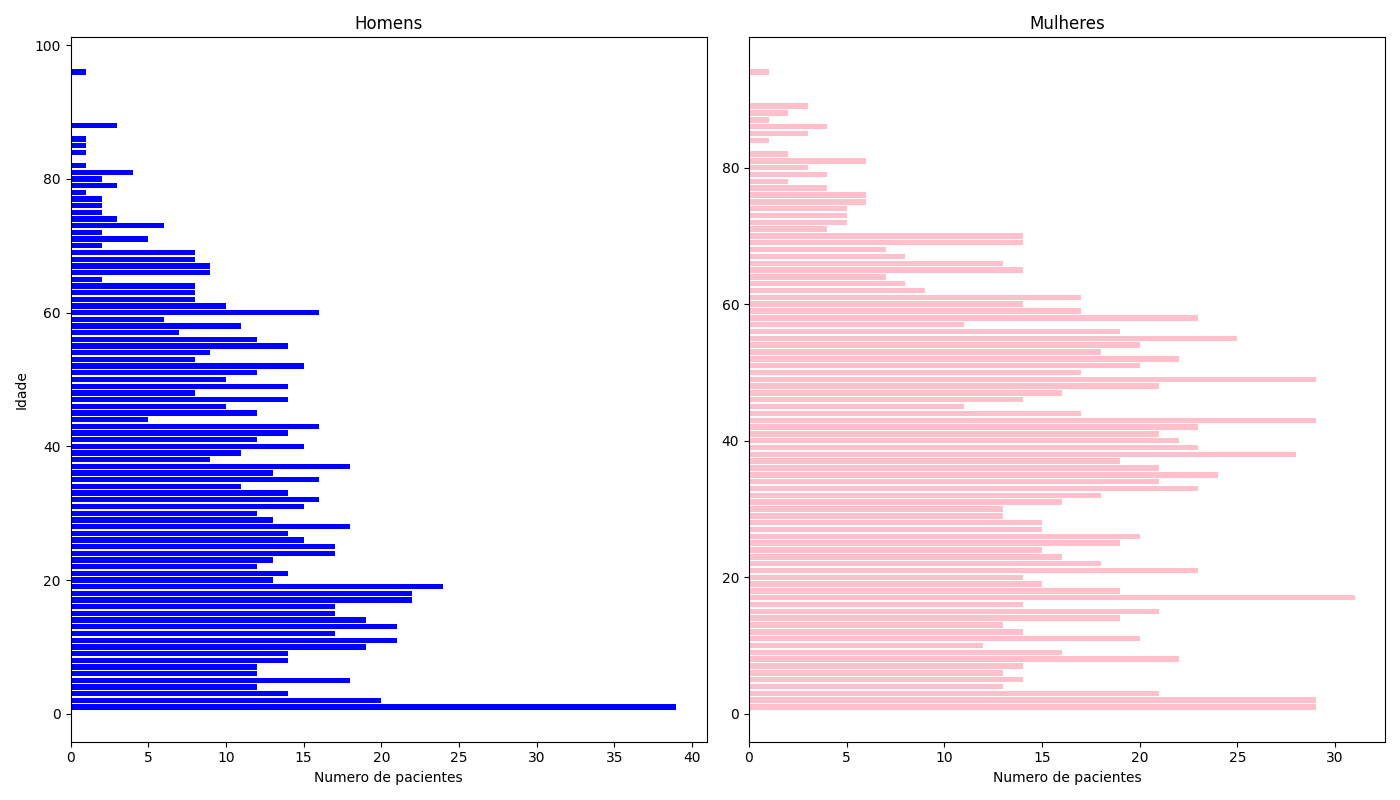
\includegraphics[width=1\textwidth]{piramide_etaria_completa.png}
    \caption{Piramide etária dos pacientes de epilepsia analisados.}
    \label{fig:piramide_etaria_completa}
\end{figure}

Observa-se que no sexo masculino há uma grande quantidade de pacientes com um ano ou menos, enquanto as mulheres têm seu valor mais destacado na faixa dos 54 anos.

Foram analisadas também particularidades sobre o tratamento utilizado. A dispensação total de medicamentos disponibilizados pelo SUS ao longo dos anos distribuiu-se da seguinte forma:

\begin{figure}[!ht]
    \centering
    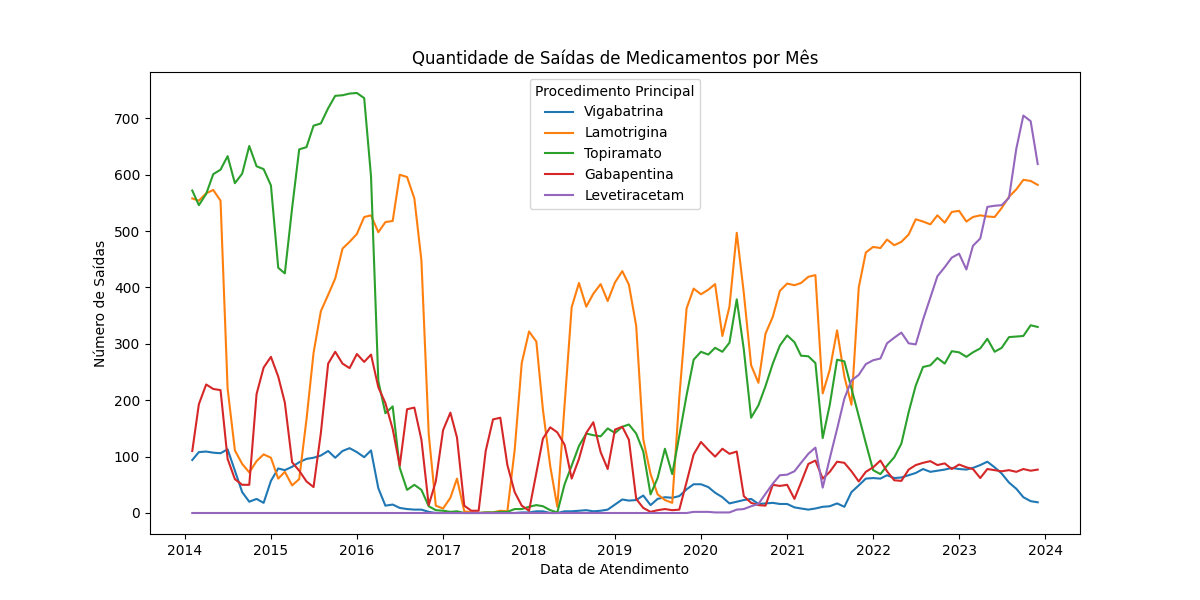
\includegraphics[width=1\textwidth]{saida_medicamentos_por_mes.png}
    \caption{Saída de medicamentos por ano.}
    \label{fig:saida_medicamentos_por_mes}
\end{figure}

Notou-se uma grande oscilação nas dispensações, provavelmente causada pela falta de abastecimento, que só conseguiu se estabilizar e manter um crescimento a partir de 2022. Observa-se a alternância em diversos períodos, onde a redução das dispensações de um medicamento era compensada pelo aumento de outro.

Quanto à distribuição dos CIDs, a maioria dos pacientes está no CID 40.0 (Epilepsia). Os três CIDs subsequentes com mais pacientes são 40.8 (Outras epilepsias), 40.2 (Epilepsia e síndromes epilépticas sintomáticas definidas por sua localização (focal) (parcial) com crises parciais complexas) e 40.4 (Outras epilepsias e síndromes epilépticas generalizadas). 


\begin{figure}[!ht]
    \centering
    
\includegraphics[width=1\textwidth]{contagem_cid_pacientes_unicos.png}
    \caption{Distribuição de CID.}
    \label{fig:contagem_cid_pacientes_unicos}
\end{figure}

\subsubsection{Modelagem}

Modelagem

\subsection{Resultados}

\subsubsection{Analise descritiva}

Como parte dos dados utilizados para construir a matriz de transição de estados, temos os gráficos que indicam os pacientes que iniciaram (Figura~\ref{fig:pacientes_iniciaram_tratamento_por_ano}) e saíram (Figura~\ref{fig:pacientes_sairam_tratamento_por_ano}) do tratamento durante o período analisado de 2014 a 2023.

\begin{figure}[!ht]
    \centering
    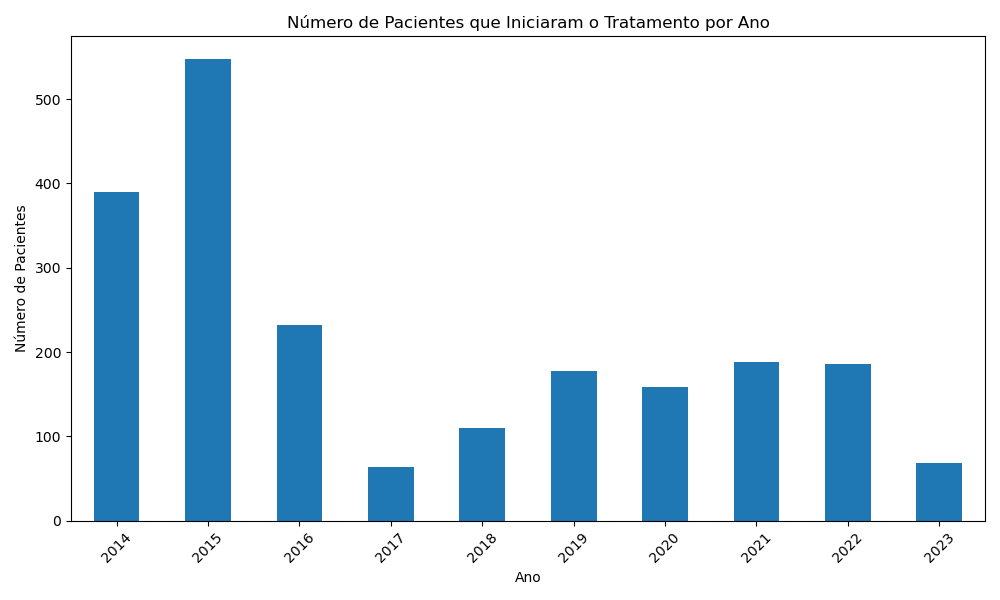
\includegraphics[width=1\textwidth]{pacientes_iniciaram_tratamento_por_ano.png}
    \caption{Pacientes que inciaram o tratamento por ano.}
    \label{fig:pacientes_iniciaram_tratamento_por_ano}
\end{figure}

Observa-se que houve um número significativamente alto de pacientes iniciando o tratamento em 2014 e 2015. Em 2017, percebe-se uma queda acentuada, possivelmente devido a problemas na disponibilidade de medicamentos. A partir de 2019, há um aumento constante no número de pacientes iniciando o tratamento, atingindo um pico em 2023. Essas variações podem indicar mudanças na política de saúde, na disponibilidade de medicamentos ou em campanhas de conscientização.

\begin{figure}[!ht]
    \centering
    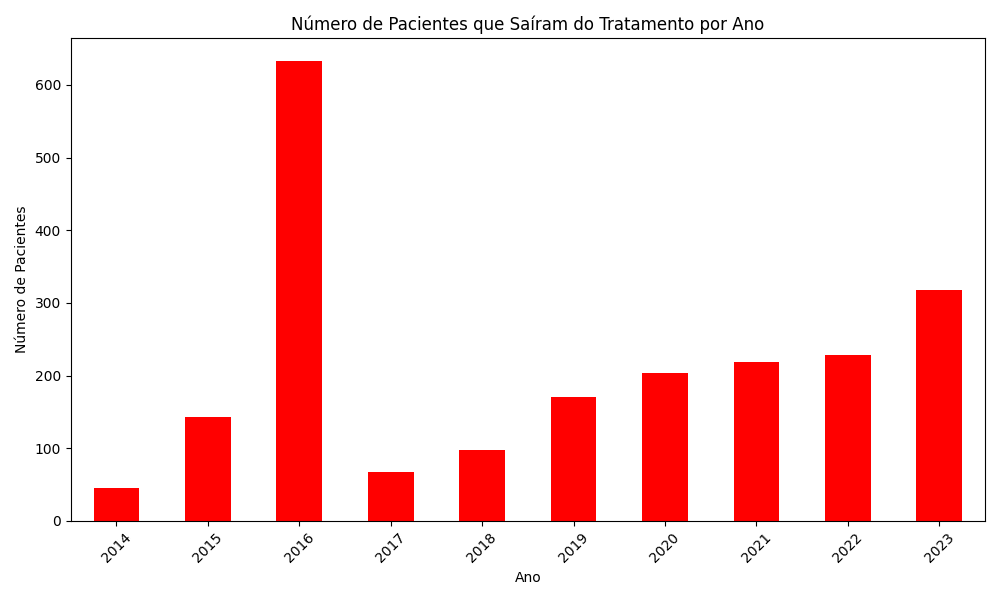
\includegraphics[width=1\textwidth]{pacientes_sairam_tratamento_por_ano.png}
    \caption{Pacientes que sairam do tratamento por ano.}
    \label{fig:pacientes_sairam_tratamento_por_ano}
\end{figure}

Quanto a saida, percebe-se que, no ano de 2017, houve uma baixa movimentação tanto de entrada quanto de saída, coincidindo com a baixa e provável falta de medicamentos vista na Figura~\ref{fig:saida_medicamentos_por_mes}. O ano de 2016 teve um pico significativo de pacientes saindo do tratamento, com flutuações nos anos subsequentes e um aumento considerável em 2023. O pico em 2016 pode estar relacionado a uma crise específica ou mudança nas diretrizes de tratamento, enquanto o aumento em 2023 pode indicar problemas recorrentes ou mudanças nas práticas de tratamento.

Além disso, observa-se que os anos 2014 e 2015 tiveram números relativamente altos de trocas de tratamento. Após uma queda em 2017, há um aumento gradual até 2023. A troca de tratamentos pode ser motivada por eficácia, efeitos colaterais ou novas opções terapêuticas se tornando disponíveis.

\begin{figure}[!ht]
    \centering
    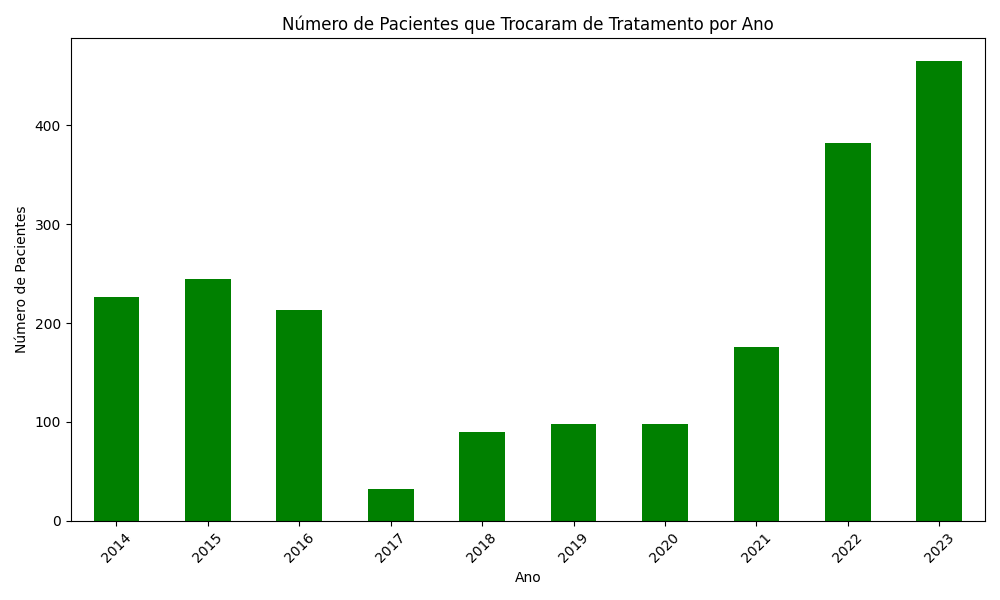
\includegraphics[width=1\textwidth]{pacientes_troca_tratamento_por_ano.png}
    \caption{Pacientes que trocaram de tratamento por ano.}
    \label{fig:pacientes_troca_tratamento_por_ano}
\end{figure}

Além disso, foram feitas pirâmides etárias com a idade da primeira retirada de cada dispensação de cada paciente, para que fosse analisada a faixa etária mais comum a cada dispensação. O resultado pode ser visto na Figura~\ref{fig:grid_piramides_etarias_medicamento} a seguir:

\begin{figure}[!ht]
    \centering
    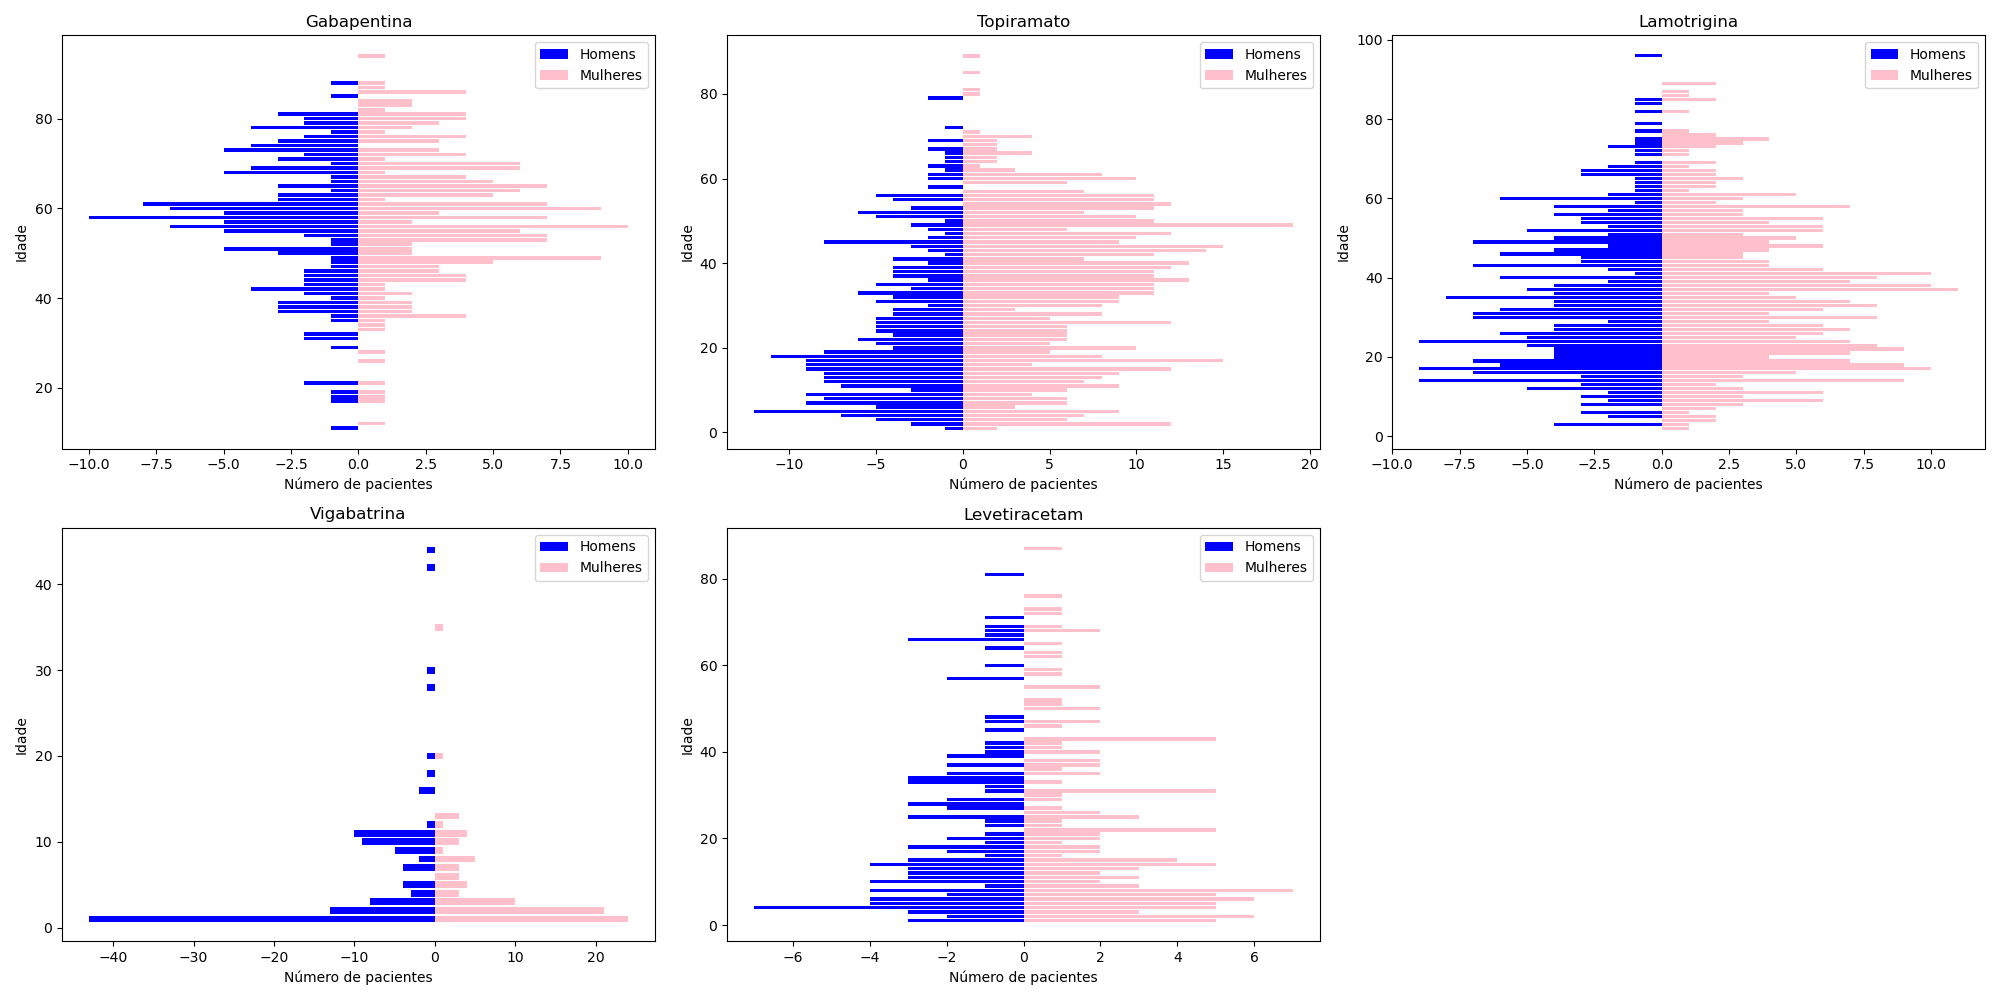
\includegraphics[width=1\textwidth]{grid_piramides_etarias_medicamento.png}
    \caption{Pirâmides etárias por dispensação.}
    \label{fig:grid_piramides_etarias_medicamento}
\end{figure}

\subsubsection{Modelagem}


Modelagem

\subsubsection{Custos}

Custos

\subsection{Discussao}

\section{Conclusao}

Parte final do artigo, na qual se apresentam as considerações correspondentes aos objetivos e/ou hipóteses.

\subsection{Citações}

As citações apresentadas no artigo seguirão as normas de apresentação de acordo com a NBR 10520:2002 ~\cite{bibliografica6023}. Para chamada das citações será adotado o sistema ``autor-dat'' em todo artigo. As chamadas incluídas na sentença devem ser em letras maiúsculas e minúsculas e, quando estiverem entre parênteses devem ser em letras maiúsculas. Nas citações diretas devem ser especificadas a(s) página(a) da fonte consultada; para citações indiretas este item é opcional. Todas as obras citadas deverão aparecer na lista de referências, e não, em notas de rodapé.

De acordo com Associação Brasileira de Normas Técnicas (~\citeyear{bibliografica6023}), ``as citações diretas, no texto, com até três linhas, devem estar contidas entre aspas duplas''.

\begin{quotation}
\noindent
As citações diretas, no texto, com mais de três linhas, devem ser destacadas com recuo de 4cm da margem esquerda, com letra menor que a do texto e sem aspas ~\cite{bibliografica6023}.
\end{quotation}

\subsection{Notas de rodapé}

As notas de rodapé devem ser utilizadas apenas para notas explicativas, ou seja, usadas para comentários, esclarecimentos ou explanações que não possam ser incluídos no texto. A numeração das notas é feita em algarismos arábicos, de forma única e consecutiva.

\subsection{Numeração progressiva}

A numeração progressiva das seções no desenvolvimento do artigo deve atender às especificações da ABNT NBR 6024:2012. As seções devem se limitar até a seção quinária e seus títulos devem ser destacados tipograficamente, de forma hierárquica, através de recursos gráficos de maiúscula, negrito, itálico ou sublinhado e outros.

\subsection{Figuras e tabelas}

Todas as figuras e tabelas devem ser numeradas em ordem crescente, na sequencia que são citadas no corpo do artigo. As figuras e tabelas devem ser exibidas preferencialmente logo após o parágrafo onde ela é citada. Todas as figuras e tabelas devem ser citadas no corpo do texto. O posicionamento da legenda é logo abaixo da figura, conforme exemplificado na Figura~\ref{fig:exampleFig1}.

\begin{figure}[!ht]
\centering
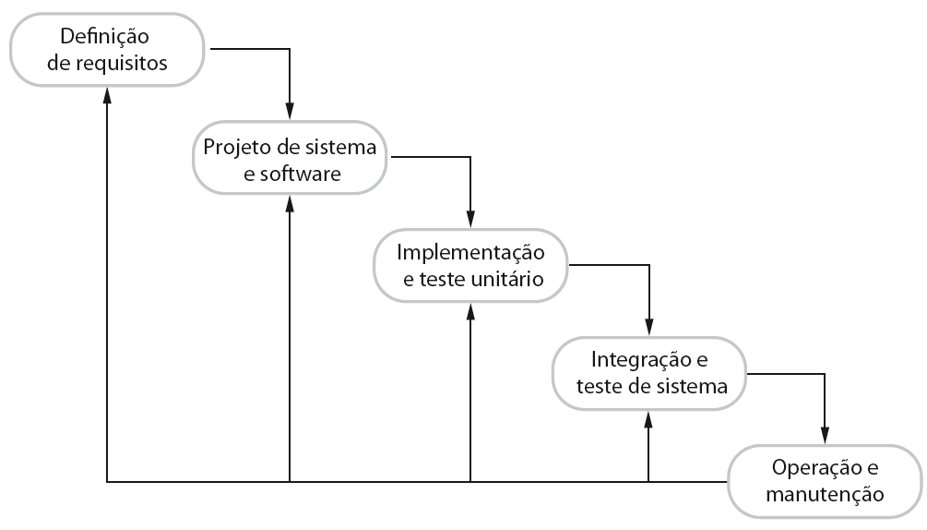
\includegraphics[width=1\textwidth]{Imagem1.png}
\caption{Modelo do processo de desenvolvimento de software em cascata. Fonte: \cite{sommerville2011software}.}
\label{fig:exampleFig1}
\end{figure}

Nas tabelas, tente evitar o uso de fundos coloridos ou sombreados e evite linhas de enquadramento grossas, dobradas ou desnecessárias. Ao relatar dados empíricos, não use mais dígitos decimais do que o garantido por sua precisão e reprodutibilidade. A legenda da tabela deve ser colocada acima da tabela (consulte a Tabela~\ref{tab:exTable1}).

\begin{table}[!ht]
\centering
\caption{Taxa de sucesso de projetos de desenvolvimento de software pelo tamanho do projeto. Fonte: \cite{clancy1995standish}.}
      \begin{tabular}{| p{3cm} | C{2cm} | C{2cm} | C{2cm} |}
        \hline
        & Bem sucedido & Deficitário & Falho \\ \hline
        Muito grande & 2 & 7 & 17 \\ \hline
        Grande & 6 & 17 & 24 \\ \hline
        Médio & 9 & 26 & 31 \\ \hline
        Pequeno & 21 & 32 & 17 \\ \hline
        Muito pequeno & 62 & 16 & 11 \\ \hline
        \textbf{TOTAL} & \textbf{100} & \textbf{100} & \textbf{100} \\ \hline
    \end{tabular}
    \label{tab:exTable1}
\end{table}

\subsection{Referências}

As referências bibliográficas devem ficar localizadas ao final do texto, contendo exclusivamente as obras citadas, ordenadas em uma única ordem alfabética e de acordo com as normas vigentes da ABNT NBR 6023/2018. Devem ser digitadas com espaçamento simples entre linhas e separadas entre si por um espaço simples em branco. O alinhamento do texto deve ser à esquerda.

A expressão ``Referências'' deve figurar de forma centralizada e não numerada, com o mesmo destaque tipográfico das seções primárias e logo após a conclusão.

Para esclarecimentos, consultar a norma correspondente.

\section{Conclusão}

Parte final do artigo, na qual se apresentam as considerações correspondentes aos objetivos e/ou hipóteses.

\newpage
\bibliography{references}

\newpage
\renewcommand{\listfigurename}{APÊNDICE A - Lista de ilustrações}
\listoffigures

\newpage
\renewcommand{\listtablename}{APÊNDICE B - Lista de tabelas}
\listoftables

\begin{appendices}
\newpage
\chapter* {APÊNDICE C}
\noindent
Os apêndices A e B devem conter a lista de ilustrações e tabelas, respectivamente. Os apêndices seguintes podem ser usados para apresentar textos elaborados pelo próprio autor, a fim de complementar a sua argumentação. Por exemplo, no caso de desenvolvimento de sistemas, podem constar nos apêndices os artefatos gerados da análise de sistemas, como protótipos de telas, casos de uso, diagramas UML, ou a lista de requisitos de negócio e de usuário.

\newpage
\chapter*{ANEXO A}
\noindent
Seção opcional. Anexos são os documentos de autoria externa, ou não elaborados pelo autor, que servem de fundamentação, comprovação ou ilustração.
\end{appendices}

\newpage
\chapter*{Agradecimentos}
\noindent
Seção opcional. Oportunidade para o(s) autor(es) registrar(em) os agradecimentos, em especial, quando o artigo recebeu ajuda financeira de alguma instituição de fomento, ou represente o resultado de um trabalho colaborativo ou multidisciplinar, envolvendo áreas externas ao Instituto de Computação.

\end{document}
